\chapter{Spatial Coherence, van Cittert--Zernike, and Intensity Interferometry}
\label{chap:e10}

\begin{chapteropening}
Chapter \ref{chap:e09} dealt with the "temporal version" of coherence: whether the same beam of light, at this instant and a little later, still remembers its own phase. This chapter moves the very same question into space. Imagine two telescopes, separated by tens of meters, hundreds of meters, or even kilometers, staring at once at the same star in the night sky. Is the light each receives "two small patches of the same wavefront"? If so, the two intensities brighten and dim together, their fluctuations synchronous; if this star subtends a large enough angle on the sky, then what the two telescopes sample are two already "offset" patches of the wavefront, their fluctuations going their separate ways, no longer synchronous. The marvel is that the degree of synchrony tells us directly how large this star is, even if, in the largest optical telescope, it is only a point. This chapter joins this chain link by link: first use pure geometry to compute "how fine an angular structure two telescopes see," then use the van Cittert--Zernike theorem to translate "what the sky looks like" into "the degree of coherence," and then, borrowing the Siegert relation of Chapter \ref{chap:e08}, explain why one can measure a star's size \emph{without combining the two beams, comparing only the jitter of their respective intensities}. Finally we will meet the weak spot of intensity interferometry (the phase is lost) and the benefit it buys in exchange: near-immunity to atmospheric jitter.
\end{chapteropening}

\section{Geometry: Two Telescopes, One Baseline, One Angular Scale}
\label{sec:e10-geometry}

Let us first set aside correlators, photons, and quantum statistics, and look at a single geometric fact, one that needs no camera at all, just a ruler and a little trigonometry.

Starlight from some direction in the sky, at a place far enough away, has had its wavefront flattened into an almost perfectly straight plane (this is the "far field"). Let the star's direction on the sky be specified by a unit vector \(\bm s\). Two telescopes stand at positions \(\bm x_1\) and \(\bm x_2\), and the vector joining them is called the \textbf{baseline}:
\[
  \bm B=\bm x_2-\bm x_1 .
\]
The same plane wavefront sweeps across one telescope first and then the other, traversing unequal path lengths. This \textbf{path difference} equals the length of the baseline projected onto the propagation direction of the starlight, that is, the dot product \(\bm B\cdot\bm s\). What truly matters for interference is the part of the baseline perpendicular to the line of sight, "lying on the plane of the sky," denoted the projected baseline \(\bm B_\perp\); the component along the line of sight merely makes the whole wavefront arrive earlier or later as a whole, without changing the transverse structure the two telescopes see.

Now focus on the fact that "the star is not a point, but a small patch of sky." Take the direction of the star's center as \(\bm s_0\), and in the \emph{local sky plane} perpendicular to the line of sight erect two orthogonal unit directions \(\hat{\bm e}_x,\hat{\bm e}_y\) (each aligned with the direction of one baseline component). Any point on the star's face, offset from the center by a small angle, is labeled by two small-angle coordinates \((l,m)\) marking this transverse offset (\(l,m\) both in radians, dimensionless, with typical values on the order of \(10^{-9}\) radians, i.e.\ milliarcseconds). Then this point's direction can be written
\[
  \bm s\approx\bm s_0+l\,\hat{\bm e}_x+m\,\hat{\bm e}_y ,
\]
where, to first order in the small angle, \(\bm s\) is still approximately normalized (the transverse offset changes \(|\bm s|\) only at second order \(\mathcal O(l^2,m^2)\), which is negligible). The extra path difference it brings, in the part that differs from the center, is
\[
  \Delta(\bm B\cdot\bm s)=B_x\,l+B_y\,m ,
\]
where \(B_x,B_y\) are the components of the projected baseline \(\bm B_\perp\) along the two orthogonal directions of the sky plane (in meters). The path difference divided by the wavelength \(\lambda\) and multiplied by \(2\pi\) is the phase difference this point brings to the two telescopes. So we naturally define a pair of \textbf{spatial frequencies}:

\begin{equation}
  u=\frac{B_x}{\lambda},\qquad v=\frac{B_y}{\lambda}.
  \label{eq:e10-uv}
\end{equation}
\begin{formulaexplain}
\(B_x,B_y\): the components of the projected baseline along the two directions of the sky plane (meters). \(\lambda\): the observation wavelength (meters). \(u,v\): the spatial frequencies measured in "numbers of wavelengths," dimensionless. The same baseline at a shorter wavelength samples finer angular structure.
\end{formulaexplain}

Why call it "spatial frequency" rather than simply "resolution"? Because \(u,v\) count "how many fringes fit into one wavelength across this baseline." It is a sampling coordinate on the Fourier plane, not the angular resolution itself. Let us substitute real numbers to feel it: take \(B=100\,\mathrm{m}\), \(\lambda=500\,\mathrm{nm}=5\times10^{-7}\,\mathrm{m}\),
\[
  \frac{B}{\lambda}=\frac{100}{5\times10^{-7}}=2\times10^{8}.
\]
Two hundred million: this is a pure number, meaning this baseline spans two hundred million wavelengths. To get the angular scale, one must \emph{invert} it:
\[
  \frac{\lambda}{B}=\frac{1}{2\times10^{8}}=5\times10^{-9}\ \mathrm{rad}.
\]
Convert radians to milliarcseconds (\(1\,\mathrm{mas}=4.848\times10^{-9}\,\mathrm{rad}\)):
\[
  5\times10^{-9}\,\mathrm{rad}=\frac{5\times10^{-9}}{4.848\times10^{-9}}\,\mathrm{mas}\approx1.0\,\mathrm{mas}.
\]
So a hundred-meter baseline, in blue-green light, innately corresponds to about 1 milliarcsecond of angular scale, already tens of times finer than the best single-aperture telescope (diffraction limit of tens of milliarcseconds). This is the whole allure of interferometry: the resolving power is set by the \emph{distance between telescopes}, not by the mirror aperture.

\section{First-Order Spatial Coherence: a Complex Arrow Across Telescopes}
\label{sec:e10-gamma12}

Geometry tells us "how fine an angular structure this baseline corresponds to," but not "whether this star is actually resolved at that angular scale." To answer the latter, we must compare the fields the two telescopes actually receive.

Recall Chapter \ref{chap:e01}: the light field at a point at a given instant can be written as an arrow rotating in the complex plane, the complex amplitude \(\mathcal E\), whose length is the amplitude and whose angle is the phase. Now the two telescopes each have an arrow, \(E_1(t)\) and \(E_2(t)\). To ask "how in step they are," the most natural quantity is to conjugate one arrow, multiply it by the other, take the time average, and normalize by each one's own intensity. This quantity is called the \textbf{first-order spatial coherence} (also called the complex visibility):

\begin{equation}
  \gamma_{12}^{(1)}
  =\frac{\big\langle E_1^{\ast}(t)\,E_2(t)\big\rangle}
        {\sqrt{\big\langle|E_1(t)|^2\big\rangle\,\big\langle|E_2(t)|^2\big\rangle}} .
  \label{eq:e10-gamma12}
\end{equation}
\begin{formulaexplain}
\(E_1,E_2\): the complex fields received by the two telescopes. The numerator \(\langle E_1^{\ast}E_2\rangle\) is the "cross-telescope field correlation," and the denominator normalizes by the square root of each one's mean intensity. The result \(\gamma_{12}^{(1)}\) is complex: the modulus \(|\gamma_{12}^{(1)}|\in[0,1]\) gives the coherence strength, and the argument gives the Fourier phase.
\end{formulaexplain}

Let us spell out each symbol. \(E_1(t),E_2(t)\): the complex amplitudes of the electric field received by the two telescopes at the same instant (in CGS the dimensions are \(\mathrm{statvolt\,cm^{-1}}\), but after normalization the units all cancel). The angle brackets \(\langle\cdot\rangle\) are the long-time average over time. In the denominator, \(\langle|E_1|^2\rangle\) is proportional to the mean intensity of the first telescope; taking the square root and multiplying by the second's exactly divides out the absolute scale of both intensities, so \(\gamma_{12}^{(1)}\) reflects only the "step," independent of which telescope collects more and which less.

Why use a complex number rather than a single real one? Because "being in step" itself carries two layers of information: \emph{how much in step} (modulus) and \emph{how much the phase has shifted} (argument). An amplitude interferometer (the kind of instrument in Chapter \ref{chap:e09} that combines the two beams via a delay line to view fringes) can read both the modulus and the argument of this complex arrow: the fringe contrast gives the modulus, the fringe position gives the argument. But the intensity interferometer to be discussed later in this chapter does \emph{not} combine beams in optics; it compares, after detection, the jitter of the two intensities, and in the end obtains only \(|\gamma_{12}^{(1)}|^2\), the argument lost. This "loss of phase" is the core feature of intensity interferometry, and we settle the account in Section \ref{sec:e10-phase}.

So what determines \(\gamma_{12}^{(1)}\)? The next section's van Cittert--Zernike theorem gives an astonishingly clean answer: it is the Fourier transform of the sky brightness distribution.

\section{The van Cittert--Zernike Theorem: the Look of the Sky Determines the Degree of Coherence}
\label{sec:e10-vcz}

Now for the most crucial derivation of this chapter. We will prove: for a "distant, internally incoherent" source, the spatial degree of coherence \(\gamma_{12}^{(1)}\) between two telescopes is exactly the \emph{normalized Fourier component} of the sky brightness distribution. This conclusion is called the van Cittert--Zernike theorem (VCZ for short), and it is the foundation of all interferometric imaging \citep{1938Phy.....5..785Z,1939Phy.....6.1129V}.

\textbf{The physical picture first.} Think of the star's face as a densely packed multitude of independent little light bulbs, each bulb in a direction \((l,m)\) with brightness \(I_\nu(l,m)\). "Internally incoherent" (spatially incoherent) means: the emissions of any two different bulbs have no phase relationship whatsoever: they are each independent thermal-radiation sources with random phase. The key is: the plane wave emitted by the \emph{same bulb} is completely coherent at the two telescopes (the same wavefront); it is only that different bulbs, because of their different directions, bring \emph{different phase differences} to the two telescopes.

\textbf{Step-by-step derivation.} To spell it out so that "the reader need supply no step," let us write the field out explicitly. The complex field received by the \(j\)-th telescope (\(j=1,2\)) is the superposition of the contributions of the bulbs in all sky directions:

\[
  E_j(t)=\int\sqrt{I_\nu(l,m)}\;a(l,m,t)\;
  \exp\!\big[-2\pi i\,(u_j\,l+v_j\,m)\big]\,\mathrm dl\,\mathrm dm .
\]

Here \(\sqrt{I_\nu(l,m)}\) is the amplitude scale of the bulb in direction \((l,m)\) (the square root of the brightness); \(a(l,m,t)\) is that bulb's \emph{complex random amplitude}: it packs in the randomly jittering phase and amplitude of the thermal-radiation source, and is a zero-mean random quantity; the exponential \(\exp[-2\pi i(u_j l+v_j m)]\) is the geometric phase of this bulb's plane wave, relative to the central direction, as it sweeps to the \(j\)-th telescope, where \((u_j,v_j)=(B_{x,j},B_{y,j})/\lambda\) is set by that telescope's position (citing the path-difference phase \(2\pi(ul+vm)\) of Section \ref{sec:e10-geometry}).

In computing the cross-telescope field correlation \(\langle E_1^{\ast}(t)E_2(t)\rangle\), multiplying the two integrals produces cross terms of all pairwise bulb pairings. To avoid confusion with the integration variables, denote the first telescope's direction as \((l_a,m_a)\) and the second's as \((l_b,m_b)\):

\[
  \big\langle E_1^{\ast}(t)E_2(t)\big\rangle
  =\int\!\!\int
  \sqrt{I_\nu(l_a,m_a)\,I_\nu(l_b,m_b)}\;
  \big\langle a^{\ast}(l_a,m_a,t)\,a(l_b,m_b,t)\big\rangle\;
  e^{\,2\pi i(u_1 l_a+v_1 m_a)}\,e^{-2\pi i(u_2 l_b+v_2 m_b)}\,
  \mathrm d\Omega_a\,\mathrm d\Omega_b ,
\]

where \(\mathrm d\Omega=\mathrm dl\,\mathrm dm\). Now invoke the \emph{incoherence condition} (the algebraic form of "independent random phases"): bulbs in different directions are mutually independent and each random, so the correlation of their complex amplitudes is nonzero only for the \emph{same bulb},

\[
  \big\langle a^{\ast}(l_a,m_a,t)\,a(l_b,m_b,t)\big\rangle
  =\delta(l_a-l_b)\,\delta(m_a-m_b) ,
\]

that is, the cross terms with \(a\neq b\) are smeared to zero by random-phase averaging (\(\langle a_a^\ast a_b\rangle=0\)), and only the diagonal terms \(a=b\) survive. Substituting this \(\delta\) function uses up the second set of integrals, setting \((l_b,m_b)=(l_a,m_a)\), and the two geometric phases combine into a \emph{difference}: \(e^{2\pi i(u_1 l+v_1 m)}e^{-2\pi i(u_2 l+v_2 m)}=e^{-2\pi i[(u_2-u_1)l+(v_2-v_1)m]}\). Denoting the spatial frequency given by the baseline difference as \((u,v)=(u_2-u_1,\,v_2-v_1)\) (exactly the \(u,v\) corresponding to the baseline \(\bm B=\bm x_2-\bm x_1\) of Section \ref{sec:e10-geometry}), we have

\[
  \big\langle E_1^{\ast}(t)E_2(t)\big\rangle
  =\int I_\nu(l,m)\,\exp\!\big[-2\pi i\,(u\,l+v\,m)\big]\,\mathrm dl\,\mathrm dm .
\]

Finally normalize by the two mean intensities per the definition Eq.~\eqref{eq:e10-gamma12}. In the denominator \(\langle|E_j|^2\rangle=\int I_\nu\,\mathrm dl\,\mathrm dm\) (for the same telescope, \(u_j=v_j\) cancel, the geometric phase is gone, and the total flux remains), the same for both telescopes, so after taking the square root it is still this total flux. Dividing numerator and denominator by the same, we obtain

\begin{equation}
  \gamma^{(1)}(u,v)
  =\frac{\displaystyle\int I_\nu(l,m)\,\exp\!\big[-2\pi i\,(u\,l+v\,m)\big]\,\mathrm dl\,\mathrm dm}
        {\displaystyle\int I_\nu(l,m)\,\mathrm dl\,\mathrm dm}.
  \label{eq:e10-vcz}
\end{equation}
\begin{formulaexplain}
Numerator: multiply the sky brightness \(I_\nu(l,m)\) by the geometric phase factor and integrate over the whole star's face: this is a two-dimensional Fourier transform. Denominator: the total flux, used to set \(\gamma^{(1)}(0,0)\) to 1. The conclusion in one sentence: \emph{the degree of coherence is the normalized Fourier component of the sky}.
\end{formulaexplain}

Let us bring each symbol down to earth. \(I_\nu(l,m)\): the specific intensity in direction \((l,m)\), commonly in units of \(\mathrm{erg\,s^{-1}\,cm^{-2}\,Hz^{-1}\,sr^{-1}}\), which can also be understood as "how bright it is per direction, per hertz of bandwidth." \(l,m\): small-angle coordinates (radians). In the exponential, \(u,l\) and \(v,m\) are paired, exactly the spatial frequency of Eq.~\eqref{eq:e10-uv} times the small angle, a pure phase, dimensionless. The denominator adds up all the star's light into the total flux, and dividing it out ensures that at zero baseline (\(u=v=0\), the two telescopes side by side) \(\gamma^{(1)}(0,0)=1\), i.e.\ "fully coherent."

The physical meaning of this formula deserves repeated savoring: \textbf{short baselines see coarse structure, long baselines see fine structure.} When \(u,v\) are small (baseline short), the phase factor barely changes over the whole star's face, the integral is approximately the total flux, and \(\gamma^{(1)}\approx1\): two telescopes close together are of course in step, because they sample the same small patch of the wavefront. As \(u,v\) grow (baseline lengthened), the phase factor begins to turn round and round over the star's face, positives and negatives cancel, the integral shrinks, and \(\gamma^{(1)}\) drops: this shows the star has been "resolved" at this angular scale. So \emph{how fast the degree of coherence drops with baseline encodes the star's size and shape}.

\textbf{Conditions of validity (check again if you cross them).} Equation~\eqref{eq:e10-vcz} is not unconditional; it used four premises, none of which may be missing:
\begin{itemize}
  \item \textbf{Source internally incoherent}: the emission phases of different points on the star's face are mutually independent; the "random-phase averaging" step above rests on this. Thermal-radiation objects almost always satisfy it.
  \item \textbf{Narrowband}: the bandwidth must be narrow, or else different wavelengths \(\lambda\) give different \(u,v\) (see Eq.~\eqref{eq:e10-uv}), smearing different spatial frequencies together.
  \item \textbf{Small field of view}: the star's subtended angle is small enough that one may use the plane \((l,m)\) coordinates and linear phase, neglecting the second-order term along the line of sight (called the \(w\)-term in radio).
  \item \textbf{Source invariant}: over the time the correlation is accumulated, the star's structure must not change significantly, or else what is averaged is something in motion.
\end{itemize}
For ordinary thermal stars and narrowband blue light in intensity interferometry, these four are generally well satisfied; but for fast transients, broadband imaging, and large-field targets, one must recheck them one by one \citep{1938Phy.....5..785Z,1939Phy.....6.1129V}.

\begin{figure}[tbp]
\centering
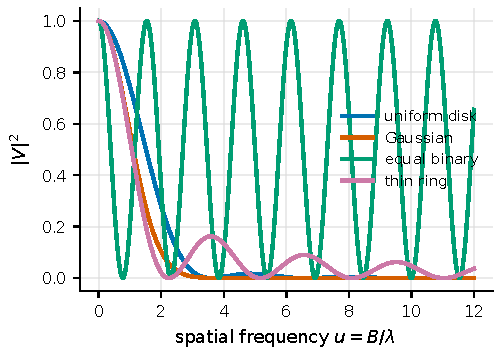
\includegraphics[width=0.88\linewidth]{figures/generated/chapter_05/ch05_vcz_visibility_models.pdf}
\caption{Different sky-brightness models leave different fingerprints on the squared visibility \(|V|^2\). A uniform disk shows Bessel-type zeros, a Gaussian source decays smoothly, equal-brightness binary stars superpose a layer of cosine oscillation, and a thin ring gives denser oscillation. What intensity interferometry directly measures is precisely these curves (their squared modulus), so "reading the curve" amounts to "guessing what the sky looks like."}
\label{fig:e10-vcz-models}
\end{figure}

\section{The Uniform Disk: Measuring a Stellar Angular Diameter from One Curve}
\label{sec:e10-disk}

The VCZ theorem gives the general formula, but the sky comes in a thousand shapes. To truly master it, one must practice on the cleanest model: the \textbf{uniform disk}. Assume the star is a circular face of angular diameter \(\theta\), with equal surface brightness everywhere inside the circle and zero outside. This is the approximation of "treating the star as a uniformly glowing coin."

\textbf{Deriving the visibility.} For a circularly symmetric brightness distribution, the two-dimensional Fourier transform degenerates into a one-dimensional Hankel transform. Let the disk radius (angular radius) be \(a=\theta/2\), and the radial spatial frequency \(q=B/\lambda\). For circular symmetry the numerator of Eq.~\eqref{eq:e10-vcz} is written
\[
  \int_0^{a} I_0\,J_0(2\pi q r)\,2\pi r\,\mathrm dr
  =2\pi I_0\int_0^{a}J_0(2\pi q r)\,r\,\mathrm dr,
\]
where \(J_0\) is the zeroth-order Bessel function, the "circularly symmetric cosine," which is exactly what remains after integrating the two-dimensional phase factor once around the circle. Here we use a standard Bessel integral identity (found in any handbook of mathematical physics):
\[
  \int_0^{a} J_0(k r)\,r\,\mathrm dr=\frac{a}{k}\,J_1(k a),
\]
taking \(k=2\pi q\). The denominator is the disk's total flux \(I_0\cdot\pi a^2\). Dividing the two:
\[
  \gamma^{(1)}
  =\frac{2\pi I_0\cdot\dfrac{a}{2\pi q}J_1(2\pi q a)}{I_0\,\pi a^2}
  =\frac{2\,J_1(2\pi q a)}{2\pi q a}.
\]
Denoting the dimensionless combination \(x\equiv 2\pi q a=2\pi\dfrac{B}{\lambda}\cdot\dfrac{\theta}{2}=\dfrac{\pi\theta B}{\lambda}\), we obtain that famous curve:

\begin{equation}
  V(B)=\frac{2\,J_1(x)}{x},\qquad x=\frac{\pi\,\theta\,B}{\lambda}.
  \label{eq:e10-disk}
\end{equation}
\begin{formulaexplain}
\(V(B)\): the visibility of a uniform disk on baseline \(B\). \(J_1\): the first-order Bessel function. \(x=\pi\theta B/\lambda\): the dimensionless "degree of resolution": the larger it is, the more the star is spread apart. As \(x\to0\), \(2J_1(x)/x\to1\) (not resolved at all).
\end{formulaexplain}

Let us account for each symbol. \(V(B)\): the visibility, dimensionless, which is the \(\gamma^{(1)}\) on this baseline (real for a disk). \(J_1(x)\): the first-order Bessel function; here we \emph{explicitly cite} this known result: the Fourier transform of a circular aperture always gives a \(J_1\)-type pattern, of the same origin as the Airy pattern of a circular hole in optics. \(\theta\): the angular diameter (radians); \(B\): the projected baseline (meters); \(\lambda\): the wavelength (meters). Most important is that combination \(x=\pi\theta B/\lambda\): for the same star, the longer the baseline or the shorter the wavelength, the larger \(x\) and the more easily resolved; for the same baseline, the larger the star, the larger \(x\) and the more sensitive.

\textbf{The first zero.} The curve \(2J_1(x)/x\) first falls to zero at the first nonzero root of \(J_1(x)=0\). This root is a known number: \(x=3.8317\). Setting \(\pi\theta B_0/\lambda=3.8317\) solves for the critical baseline:
\[
  B_0=\frac{3.8317}{\pi}\cdot\frac{\lambda}{\theta}=1.2197\,\frac{\lambda}{\theta}\approx1.22\,\frac{\lambda}{\theta}.
\]

\begin{equation}
  B_0\approx\frac{1.22\,\lambda}{\theta}.
  \label{eq:e10-null}
\end{equation}
\begin{formulaexplain}
\(B_0\): the baseline (meters) at which the visibility first drops to zero. \(\lambda\): wavelength, \(\theta\): angular diameter. It marks the telescope separation needed to "just resolve the star to the first dark fringe," looking exactly like the single-aperture diffraction limit \(1.22\lambda/D\), only with the aperture \(D\) replaced by the baseline \(B\).
\end{formulaexplain}

\textbf{Substituting real numbers.} Take the blue light \(\lambda=416\,\mathrm{nm}\) commonly used by VERITAS and MAGIC, and see how long a baseline several stellar sizes require:
\[
  \theta=0.5\,\mathrm{mas}=0.5\times4.848\times10^{-9}\,\mathrm{rad}=2.424\times10^{-9}\,\mathrm{rad},
\]
\[
  B_0=1.22\times\frac{416\times10^{-9}}{2.424\times10^{-9}}
  =1.22\times171.6\,\mathrm{m}\approx210\,\mathrm{m}.
\]
Similarly, \(\theta=1\,\mathrm{mas}\) needs only about \(105\,\mathrm{m}\), and \(\theta=0.2\,\mathrm{mas}\) needs about \(520\,\mathrm{m}\). These few numbers explain the whole span of instrument history: the Narrabri intensity interferometer used a variable baseline of 10--188 m, enough to measure those brighter, sub-milliarcsecond stars; but to reach down to tens of microarcseconds, one must go to kilometer-scale baselines, which is exactly the motivation for using atmospheric Cherenkov telescope arrays (VERITAS, MAGIC, the future CTAO) as intensity interferometers \citep{1967MNRAS.137..375H,2020NatAs...4.1164A}.

\begin{figure}[tbp]
\centering
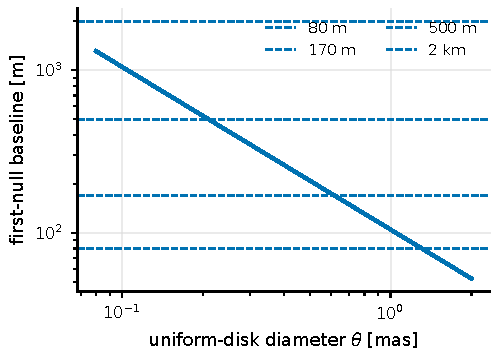
\includegraphics[width=0.86\linewidth]{figures/generated/chapter_05/ch05_uniform_disk_resolution.pdf}
\caption{The first-zero baseline of a uniform disk at \(\lambda=416\,\mathrm{nm}\) versus angular diameter. A 0.5 mas star needs about 210 m to reach its first zero, while a target of order 0.1 mas requires kilometer-scale baselines: this is why long-baseline Cherenkov arrays are so attractive for blue-light intensity interferometry.}
\label{fig:e10-disk-resolution}
\end{figure}

A practical reminder: what carries the most information in observing is often \emph{not} the zero itself, but the "descending region" before the zero. At short baselines, the curves of various angular diameters all cling to \(|V|^2\approx1\), indistinguishable; after the zero, \(|V|^2\) is too low, and systematic errors and background easily drown the signal; only the descending region has both appreciable signal and sensitivity to \(\theta\). So the first thing in designing an observation is to plot the \(|V(B)|^2\) of the target model and let the baselines cover this descending region (see Fig.~\ref{fig:e10-vcz-models}).

\section{Spatial HBT: No Beam Combining, Just Whether Intensity Jitter Is Synchronous}
\label{sec:e10-hbt}

Up to here we have kept talking about first-order coherence \(\gamma^{(1)}\) and the complex visibility: that is what an amplitude interferometer measures, requiring the two beams to be carefully combined in optics. Intensity interferometry takes another route: it does not combine beams at all, and only after detection compares whether the jitter of the two \emph{intensities} is synchronous. On what grounds can this too measure \(|V|\)? The answer is the Siegert relation of Chapter \ref{chap:e08}.

In Chapter \ref{chap:e08} we established, for the same light path at different instants, \(g^{(2)}=1+\zeta|g^{(1)}|^2\): the intensity of thermal (chaotic) light clumps together (photon bunching), and the strength of the bunching is proportional to the squared modulus of the first-order degree of coherence. This relation holds just as well for "two light paths, same instant," as long as the time channel is replaced by the spatial channel:

\begin{equation}
  g_{12}^{(2)}(0)-1=\zeta\,\big|\gamma_{12}^{(1)}\big|^2=\zeta\,\big|V(B)\big|^2 .
  \label{eq:e10-siegert}
\end{equation}
\begin{formulaexplain}
\(g_{12}^{(2)}(0)-1\): the "excess" of the zero-delay intensity correlation of the two telescopes (the extra clumping relative to accidental coincidence). \(\zeta\): the dilution factor (time response, bandwidth, polarization, and background together lower the bunching height). \(|V(B)|^2\): the squared visibility, exactly the celestial structure we want.
\end{formulaexplain}

Let us explain each symbol. \(g_{12}^{(2)}(0)\): the normalized second-order correlation of the two intensities at zero time delay; subtracting 1 gives the excess relative to the "completely random, uncorrelated" baseline. \(\zeta\) (dimensionless, between 0 and 1): bundles in everything that "flattens the bunching peak": the finite detector time width, the finite optical bandwidth, unselected polarization, background-light dilution. \(|\gamma_{12}^{(1)}|^2\): for thermal light / Gaussian chaotic light, it equals \(|V(B)|^2\). This formula is the heart of spatial HBT (Hanbury Brown--Twiss): \textbf{the degree of synchrony of the intensity jitter of the two telescopes directly gives the squared visibility}, with no beam combining anywhere \citep{1956Natur.177...27B}.

\textbf{The observation model.} On a real machine, data analysis often writes Eq.~\eqref{eq:e10-siegert} as a model that separates the three things "instrument, background, celestial object." This step is really just \emph{writing out clearly the lumped dilution factor \(\zeta\) of Eq.~\eqref{eq:e10-siegert}}, splitting it into \(\zeta=N_0\,f_1 f_2\): \(N_0\) collects the instrument-side dilution (detector time response, bandwidth, polarization, i.e.\ the term Eq.~\eqref{eq:e10-n0} below), and \(f_1 f_2\) collects the background-side dilution (the fraction of target photons out of the total counts of the two telescopes). So the dilution factor has not vanished; it is only split into "instrument \(\times\) background," each of which can be calibrated separately:

\begin{equation}
  C_{12}(B)\equiv g_{12}^{(2)}(0)-1=N_0\,f_1 f_2\,\big|V(B)\big|^2 .
  \label{eq:e10-model}
\end{equation}
\begin{formulaexplain}
\(C_{12}\): the measured correlation-peak height. \(N_0\): the zero-baseline instrument response (the bunching height that should occur when the star is not spatially resolved). \(f_1,f_2\): the fractions of target photons out of the total counts in the two telescopes. \(|V|^2\): the celestial structure term. The product of the three cleanly separates instrument, background, and sky.
\end{formulaexplain}

Symbol by symbol: \(C_{12}(B)\) is the correlation-peak amplitude on baseline \(B\) (dimensionless); \(N_0\) is the \emph{zero-baseline} correlation amplitude, i.e.\ the bunching height that should occur when the two telescopes are side by side and the star is completely unresolved (\(|V|=1\)), which collects in all the post-detection instrument effects; \(f_1,f_2\) (dimensionless, \(\le1\)) are the fractions of light truly from the target in each telescope: moonlight, night-sky light, and neighboring stars pull it down; \(V(B)\) is the normalized visibility given by Eq.~\eqref{eq:e10-disk} (or a more complex model). This product structure lets the analysis be calibrated term by term: \(|V|^2\) varies with baseline, \(f_1f_2\) varies with background, and \(N_0\) is the instrument's "identity card."

\textbf{How small is the zero-baseline amplitude.} For unpolarized thermal light, if the detector has an effective time width \(\Delta t_{\rm eff}\) and an optical bandwidth \(\Delta\nu\), the order of magnitude of the zero-baseline amplitude is

\begin{equation}
  N_0\sim\frac{1}{2\,\Delta\nu\,\Delta t_{\rm eff}},\qquad
  \Delta\nu\simeq\frac{c\,\Delta\lambda}{\lambda^2}.
  \label{eq:e10-n0}
\end{equation}
\begin{formulaexplain}
\(N_0\): the bunching-peak height when the star is unresolved. \(\Delta\nu\): the optical frequency bandwidth (Hz). \(\Delta t_{\rm eff}\): the electronic effective time width (s). The \(2\) in the denominator is the dilution from unselected polarization (two polarization modes). The wider the bandwidth and the slower the time response, the lower the thermal-light bunching peak is averaged down.
\end{formulaexplain}

Physically this is easy to understand (recall from Chapter \ref{chap:e02} that bandwidth and coherence time are reciprocals): bunching is only "visible" within one coherence time \(\tau_c\sim1/\Delta\nu\), while the detector must spend \(\Delta t_{\rm eff}\) integrating. When the detector is much slower than the coherence time (\(\Delta t_{\rm eff}\gg\tau_c\)), a single integration packs in \(\sim\Delta t_{\rm eff}/\tau_c=\Delta\nu\,\Delta t_{\rm eff}\) mutually uncorrelated coherence blocks, and the bunching signal is thinned by averaging over so many blocks, so \(N_0\) is inversely proportional to this large number.

\textbf{Substituting VERITAS's real parameters} (\(\lambda=416\,\mathrm{nm}\), \(\Delta\lambda=13\,\mathrm{nm}\), \(\Delta t_{\rm eff}\sim4\,\mathrm{ns}\)): first compute the bandwidth
\[
  \Delta\nu\simeq\frac{c\,\Delta\lambda}{\lambda^2}
  =\frac{(3\times10^8)\,(13\times10^{-9})}{(416\times10^{-9})^2}
  =\frac{3.9}{1.73\times10^{-13}}\ \mathrm{Hz}\approx2.3\times10^{13}\,\mathrm{Hz},
\]
then substitute into \(N_0\):
\[
  N_0\sim\frac{1}{2\,(2.3\times10^{13})\,(4\times10^{-9})}
  =\frac{1}{1.8\times10^{5}}\approx5\times10^{-6}.
\]
The order of magnitude is a few parts per million. The \(N_0\approx1.25\times10^{-6}\) obtained by fitting the real machine is slightly lower than the crude estimate, because the real filter shape, electronic response, and system efficiency further suppress the peak. In any case, the conclusion is sobering: \textbf{the bunching peak of thermal light is only of order one part in a million}, and to measure a star on such a low signal relies on long-duration accumulation and stringent calibration of \(N_0\) (Fig.~\ref{fig:e10-zero-baseline}) \citep{2020NatAs...4.1164A}.

\begin{figure}[tbp]
\centering
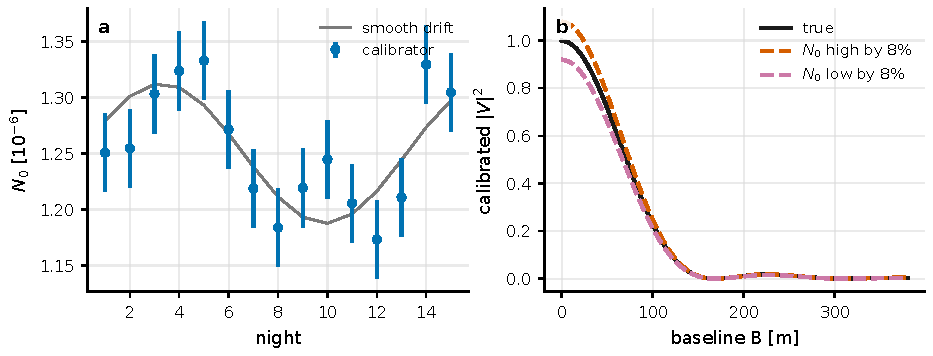
\includegraphics[width=0.92\linewidth]{figures/generated/chapter_05/ch05_zero_baseline_calibration.pdf}
\caption{The calibration of the zero-baseline amplitude \(N_0\) carries directly over onto \(|V|^2\). Left: the nightly \(N_0\) drift given by calibration stars. Right: if \(N_0\) is 8\% too high or too low, \emph{all} baselines' \(|V|^2\) are stretched as a whole, pushing the fits of angular diameter, limb darkening, or oblateness toward wrong values. This explains why \(N_0\) is the most critical systematic in intensity interferometry.}
\label{fig:e10-zero-baseline}
\end{figure}

\section{Missing Phase: a Weak Spot, and Also an Amulet}
\label{sec:e10-phase}

Intensity interferometry measures only \(|V|^2\) (that squared modulus in Eq.~\eqref{eq:e10-model}), throwing away the argument (Fourier phase) of the complex visibility \(\gamma_{12}^{(1)}\). This brings an ambiguity of principle.

\textbf{Mirror degeneracy.} Consider a brightness distribution \(I(l,m)\) and its mirror image \(I(-l,-m)\), flipped about the center. Taking the Fourier transform per Eq.~\eqref{eq:e10-vcz}, the Fourier transform of a real brightness distribution satisfies \(\gamma(-u,-v)=\gamma^{\ast}(u,v)\) (because \(I\) is real); and the Fourier transform of the mirror distribution is exactly the complex conjugate of the original. Taking the squared modulus, complex conjugation does not change the modulus, so
\[
  \big|V_{\text{original}}(u,v)\big|^2=\big|V_{\text{mirror}}(u,v)\big|^2 .
\]
Two skies that look different give \emph{exactly the same} \(|V|^2\): an instrument that measures only the squared modulus cannot distinguish them (Fig.~\ref{fig:e10-phase-ambiguity}). This is why "imaging directly from \(|V|^2\)" is a hard matter requiring extra information (two-dimensional \(u,v\) coverage, physical priors, third-order correlation, or phase-retrieval algorithms), and we leave true imaging to Chapter \ref{chap:e11}.

\begin{figure}[tbp]
\centering
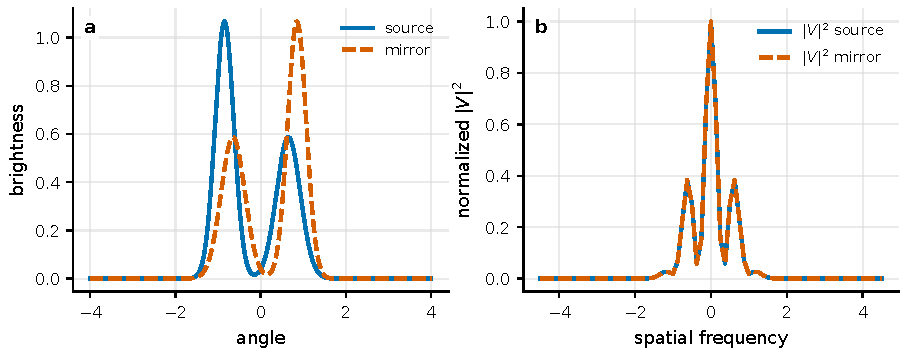
\includegraphics[width=0.92\linewidth]{figures/generated/chapter_05/ch05_phase_ambiguity.pdf}
\caption{Measuring only \(|V|^2\) loses the Fourier phase. Left: a source and its mirror source, with clearly different brightness distributions. Right: the \(|V|^2\) of the two coincide completely. To image, intensity interferometry must break such degeneracies through two-dimensional \(u,v\) coverage, physical priors, third-order (closure) correlation, or phase-retrieval algorithms.}
\label{fig:e10-phase-ambiguity}
\end{figure}

\textbf{What does losing the phase buy?} The answer is: near-immunity to optical path and atmospheric jitter, which is exactly the fundamental reason Cherenkov telescopes can do interferometry. An amplitude interferometer must combine the two beams in optics to view fringes, and so must stabilize the \emph{optical path} of the two light paths to a small fraction of a wavelength (of order tens of nanometers); but atmospheric turbulence makes the wavefront fluctuate ceaselessly, adding to each telescope a random, fast-jittering optical-path offset, termed the \textbf{piston phase}. Piston is fatal to amplitude interferometry, jittering the fringes away.

Intensity interferometry, however, hardly cares about it. The reason is: it compares whether the jitter of the two \emph{intensities} is synchronous, needing only to align the two \emph{electrical signals} in time to a small fraction of the detection response time. For a \(1\,\mathrm{GHz}\) electronic bandwidth, the time resolution is about 1 ns, and the corresponding optical-path tolerance is \(c\times1\,\mathrm{ns}\approx30\,\mathrm{cm}\): a path error of centimeters to tens of centimeters would be needed to noticeably reduce the correlation. Atmospheric piston's nanometer-to-micron optical-path jitter is not even a fraction of this tolerance. In other words, \textbf{intensity interferometry, at the cost of "losing the phase," buys the huge convenience of "not fearing the atmosphere and not needing precise optical path."} For exactly this reason, Cherenkov telescopes, whose optical image quality is far below that of professional interferometers but which have large apertures and fast detectors, turn out to be ideal intensity-interferometry arrays \citep{2006ApJ...649..399L,2024MNRAS.529.4387A}.

\section{Chapter Summary}
\label{sec:e10-summary}

\begin{itemize}
  \item \textbf{Geometry sets the angular scale.} The projected baseline \(\bm B_\perp\) gives the path difference \(\bm B\cdot\bm s\), and the spatial frequencies \(u=B_x/\lambda,\ v=B_y/\lambda\) are dimensionless "numbers of wavelengths." A hundred-meter baseline in blue-green light corresponds to about 1 mas (\(B/\lambda=2\times10^8\), inverted \(\lambda/B\approx1\,\mathrm{mas}\)). The resolving power is set by the baseline, not the aperture.
  \item \textbf{The degree of coherence is a complex arrow.} The first-order spatial degree of coherence \(\gamma_{12}^{(1)}=\langle E_1^\ast E_2\rangle/\sqrt{\langle|E_1|^2\rangle\langle|E_2|^2\rangle}\): the modulus gives the coherence strength, the argument gives the Fourier phase.
  \item \textbf{The van Cittert--Zernike theorem.} The \(\gamma^{(1)}(u,v)\) of an incoherent far-field source is the Fourier component of the normalized sky brightness (Eq.~\eqref{eq:e10-vcz}). Short baselines see coarse structure, long baselines see fine structure. Four conditions for validity: source internally incoherent, narrowband, small field of view, source invariant.
  \item \textbf{The uniform disk.} \(V(B)=2J_1(x)/x,\ x=\pi\theta B/\lambda\) (first-order Bessel function); the first zero \(x=3.8317\) gives \(B_0\approx1.22\lambda/\theta\). 416 nm, 0.5 mas \(\Rightarrow\) about 210 m. The most informative is the descending region before the zero.
  \item \textbf{Spatial HBT.} Carry the Siegert relation of Chapter \ref{chap:e08} over to the spatial channel: \(g_{12}^{(2)}(0)-1=\zeta|V(B)|^2\); no beam combining, just the synchrony of intensity jitter measures \(|V|^2\). The observation model \(C_{12}=N_0 f_1 f_2|V|^2\), zero-baseline amplitude \(N_0\sim1/(2\Delta\nu\Delta t_{\rm eff})\); VERITAS parameters give about \(5\times10^{-6}\), measured \(1.25\times10^{-6}\).
  \item \textbf{Missing phase is a double-edged sword.} Measuring only \(|V|^2\), the mirror brightness distribution \(I(-l,-m)\) gives the same \(|V|^2\) (degeneracy); but the price buys immunity to optical path / atmospheric piston, which is exactly why Cherenkov telescopes can do interferometry. Imaging is left to Chapter \ref{chap:e11}.
\end{itemize}

\medskip
\noindent\textbf{Questions to Ponder.}
\begin{itemize}
  \item If the observation wavelength is changed from 416 nm to the red light of 640 nm, will the first-zero baseline of the same 0.5 mas star become longer or shorter? To how many meters?
  \item If the target-photon fraction in the two telescopes drops from 70\% to 50\%, to what fraction of its original value is the correlation peak in Eq.~\eqref{eq:e10-model} suppressed? To recover the same significance, by roughly how many times must the integration time be increased (recall SNR grows only as the square root of time)?
  \item Why is "narrowband" a necessary condition of the VCZ theorem? If the bandwidth is very wide, what goes wrong with Eq.~\eqref{eq:e10-uv}?
\end{itemize}
